% This is LLNCS.DEM the demonstration file of
% the LaTeX macro package from Springer-Verlag
% for Lecture Notes in Computer Science,
% version 2.4 for LaTeX2e as of 16. April 2010
%
\documentclass{llncs}
\usepackage{amsopn} % DeclareMathOperator
\usepackage{amsmath} % bmatrix
\usepackage{graphicx} % include graphics

\DeclareMathOperator{\Var}{Var}
\newcommand{\effectvector}{Y}
\newcommand{\effect}[1][i]{\effectvector_{#1}}
\newcommand{\vareffect}[1][i]{V_{\effect[#1]}}
\newcommand{\zeffect}[1][i]{Z_{#1}}
\newcommand{\nStudies}{k}
\newcommand{\varCombined}{\sigma^2_{C}}
\newcommand{\varBetween}{\tau^2}
\newcommand{\varWithinCommon}{\sigma^2}
\newcommand{\sampleSize}[1][i]{n_{#1}}
\newcommand{\varWithin}[1][i]{\sigma^2_{#1}}




\usepackage{makeidx}  % allows for indexgeneration
%
\begin{document}
%
\frontmatter          % for the preliminaries
%
\pagestyle{headings}  % switches on printing of running heads
% \addtocmark{Hamiltonian Mechanics} % additional mark in the TOC
%
%
\mainmatter              % start of the contributions
%
\title{Is Z enough? Impact of Meta-Analysis using only Z/T images in lieu of estimates and standard errors}
%
\titlerunning{Running title}  % abbreviated title (for running head)
%                                     also used for the TOC unless
%                                     \toctitle is used
%
\author{Camille Maumet\inst{1} \and TODO pain
\and Thomas E. Nichols\inst{1,2}}
%
\authorrunning{Camille Maumet et al.} % abbreviated author list (for running head)
%
%
\institute{Warwick Manufacturing Group, The University of Warwick, Coventry, UK.\\
\and
Statistics Department, The University of Warwick, Coventry, UK.}

\maketitle              % typeset the title of the contribution

\begin{abstract}
The abstract should summarize the contents of the paper
using at least 70 and at most 150 words. It will be set in 9-point
font size and be inset 1.0 cm from the right and left margins.
There will be two blank lines before and after the Abstract. \dots
\keywords{computational geometry, graph theory, Hamilton cycles}
\end{abstract}
%
\section{Introduction}
While most neuroimaging meta-analyses are based on peak coordinate data, the best practice method is an Intensity-Based Meta-Analysis (IBMA) that combines the effect estimates and their standard errors (E+SE's, aka COPE \& sqrt-VARCOPE) from each study [5]. Various efforts are underway to facilitate sharing of neuroimaging data to make such IBMA's possible (see, e.g. [2]), but the emphasis is usually on T-statistics and E+SE's are difficult to use in practice; for example, an analysis of E+SE's requires knowledge of the data, design and contrast scaling. However a meta-anlaysis based on T-statistic images is sub-optimal and discouraged in (non-imaging) meta-analysis [1], as the units of the meta-analysis are, say, ``BOLD significance'' instead of ``\% BOLD change''.


Given a set of $k$ studies, we can face different configuration of data sharing, and hence for each study $i$ having available for meta-analysis:
\begin{enumerate}
	\item the contrast estimates $\effect$ and contrast variance estimates $\vareffect$.
	\item the contrast estimates $\effect$.	
	\item the standardized statistical maps $\zeffect$.		
\end{enumerate}

Depending on how much is shared different strategies can be used to combine the available results into a meta-analysis.

Here we compare the use of IMBA using only T-statistics to use of E+SE's. Using 21 studies of pain in control subjects, we compare the best-practice analysis to two approaches using only T-statistics, Stouffer's [7] and weighted Z-score [4], the latter accounting for differing study sample size.

\section{Methods}
\subsection{Theory}
Given a set of $k$ studies, we denote for each study $i$: its contrast estimate by $\effect$, its contrast variance estimate by $\vareffect$, its standardized statistical map by $\zeffect$ and its sample size by $n_i$.		

\paragraph{Combining contrast estimates and their standard error}

The gold standard approach to combine contrast estimates and their standard errors is to input them into a GLM, creating effectively the third-level of a hierarchical model (level 1, subject; level 2, study; level 3: meta-analysis). The general formulation is provided in the following equation:

\begin{equation}
	\effectvector = X \beta + \epsilon
	\label{eq_meta_GLM}
\end{equation}

where $\beta$ is the meta-analytic parameter to be estimated, $Y = [\effect[1] \ldots \effect[\nStudies] ]^t$ is the vector of contrast estimates and $\epsilon \sim \mathcal{N}(0,W)$ is the residual term. Eq.~\eqref{eq_meta_GLM} can be solved by weighted least square giving:

% TODO add contrast

\begin{eqnarray}
	\hat \beta  &=& (X^t W X)^{-1} X^t W \effectvector \\
	\Var(\hat \beta)  &=& (X^t W X)^{-1}
	\label{eq_WLS}
\end{eqnarray}

In a fixed-effects model (i.e. assuming no between-study variances), we have $W = diag( \varWithin[1] \ldots \varWithin[\nStudies] )$ where $\varWithin$ denotes the contrast variance for study $i$. In a random-effects model, we have $W = diag( \varWithin[1] + \varBetween \ldots \varWithin[\nStudies] + \varBetween )$ where $\varBetween$ denotes the between-studies variance. Approximating $\varWithin$ by $\vareffect[i]$ and given $\hat\varBetween$ an estimate of $\varBetween$ we obtain the statistics detailed in table~\ref{stat_table} for one sample tests.

\begin{table}[h]
\begin{center}
\begin{tabular}{ccc}
						& Statistic			& Disbribution under H$_0$ \\
\hline						
GLM FFX 				& $ \displaystyle \frac{1}{ \sqrt{\sum_{i=1}^\nStudies 1/\vareffect }} \sum_{i=1}^\nStudies \frac{\effect}{\vareffect}$ & $\mathcal{T}_{ (\sum_{i=1}^\nStudies n_i - 1) - 1}$ \\
GLM MFX 				& $ \displaystyle \frac{1}{ \sqrt{\sum_{i=1}^\nStudies 1/ (\vareffect + \hat\varBetween) }} \sum_{i=1}^\nStudies \frac{\effect}{\vareffect + \hat\varBetween}$ & $\mathcal{T}_{\nStudies - 1}$ \\
GLM RFX	 				& $ \displaystyle \frac{1}{\widehat\varCombined / \sqrt{\nStudies}} \sum_{i=1}^\nStudies \frac{\effect}{\nStudies}$ & $\mathcal{T}_{\nStudies - 1}$ \\
Fisher's 				& $\displaystyle -2 \sum_{i=1}^{\nStudies} \ln( \Phi(-\zeffect) ) )$ & $\chi^2_{(2\nStudies)}$\\
Stouffer's 				& $\displaystyle  \frac{\sum_{i=1}^\nStudies \zeffect}{\sqrt{\nStudies}}$ & $\mathcal{N}(0,1)$ \\
Stouffer's MFX			& $\displaystyle  \frac{\sum_{i=1}^\nStudies \zeffect}{\sqrt{\nStudies} \hat \sigma}$ & $\mathcal{T}_{\nStudies-1}$ \\
Optimally weighted-Z	& $\displaystyle  \frac{\sum_{i=1}^\nStudies  \sqrt{n_i} \zeffect}{\sqrt{\sum_{i=1}^\nStudies n_i}}$ & $\mathcal{N}(0,1)$ \\
\hline 

\end{tabular}
\end{center}
\caption{Statistics for one-sample meta-analysis tests and distributions under the null hypothesis.}
\label{stat_table}
\end{table}

\paragraph{Combining contrast estimates}
In the absence of standard error, the contrast estimates $\effect$ can be combined by assuming that the within-study variance $\varWithin$ is roughly constant ($\varWithin \simeq \sigma^2 \; \forall \, 1 \le i \le \nStudies $) or a negligible by comparison to the between-study variance($\varWithin \ll \varBetween \; \forall \, 1 \le i \le \nStudies $). Then $W = diag( \varCombined \ldots \varCombined )$ where $\varCombined$ is the combined within and between-stubject variance such as $\varCombined \simeq \varBetween$ or $\varCombined \simeq \varBetween + \varWithinCommon$. Eq.~\eqref{eq_meta_GLM} can be solved by ordinary least square giving:

\begin{eqnarray}
	\hat \beta  &=& (X^t X)^{-1} X^t \effectvector \\
	\Var(\hat \beta)  &=& (X^t W X)^{-1}
	\label{eq_OLS}
\end{eqnarray}

Given $\hat\varCombined$ an estimate of $\varCombined$ we obtain the statistics detailed in table~\ref{stat_table} for one sample tests.

\paragraph{Combining standardised statistics} 
In the presence of standardiseds statistical estimates, Fisher proposed to combine the associated p-values~\cite{Fisher1932}. Stouffer's proposed to combine directly the standardised statistic~\cite{Stouffer1949}. In \cite{Zaykin2011} following \cite{Liptak1958}, the author proposed a weighted method that weights each study's $\zeffect$ by the square root of its sample size [3,7]. All these statistics, assuming fixed-effects and suited only for one-sample tests only are presented in table~\ref{stat_table}.

As suggested in~\cite{Salimi-khorshidi2009}, to get a kind of MFX with Stouffer's approach, the standardised statistical estimates $\zeffect$ can be combined in an OLS analysis. The corresponding estimate, referred as Stouffer's MFX is also provided in~\ref{stat_table}

\subsection{Experiments}

\subsubsection{Simulations}
To verify the validity of each estimator under the null hypothesis we estimated the false positive rate at $p<0.05$ uncorrected. For each meta-analysis, we simulated a contrast estimate a variance estimates such as:
\begin{eqnarray}
	\effect &\sim& \mathcal{N}(0, \frac{\varWithin}{\sampleSize}+\varBetween) \\
	\vareffect &\sim& \frac{\varWithin}{\sampleSize-1} \chi^2_{(\sampleSize-1)}%
\end{eqnarray}
where $\varWithin \in [1/2, 1, 2, 4]$ is the within-study variance, $\varBetween \in [0, 1]$ is the between-study variance (fixed-effects if $\varBetween$ is $0$, random-effects otherwise). We simulated different number of studies: $\nStudies \in [5, 10, 25, 50]$ and for a given meta-analysis, the number of subjects per studies $n$ was selected such as we would have varying number of subjects in a common range for neuroimaging studies. In each simulated meta-analysis we simulated one study with exactly $20, 25, 10$ and $50$ subjects. For the remaining studies the number of subjects were drawn from uniform distributions a quarter from $\mathcal{U}(11,20)$, a quarter from $\mathcal{U}(26,50)$ and the remaining from $\mathcal{U}(21,25)$. A total of 32 parameter sets (4 $\varWithin$ x 2 $\varBetween$ x 4 $\nStudies$) was therefore tested, 71 repeats with 5041 samples per repeats were simulated.


\subsubsection{Real data}

We first compared the Z-scores obtained by the three approaches using a Bland-Altman plot. Then, as results are usually presented as a thresholded map, we computed the dice similarity score between thresholded maps obtained with Stouffer's and weighted-Z FFX with FLAME FFX for three (uncorrected) thresholds: p < 0.001, 0.01 and 0.05. Finally, as results are best reported using a multiple comparison correction, we defined ground truth activations as the FLAME FFX analysis FDR-corrected at a threshold of p<0.05 and plotted Receiver-Operating-Characteristics (ROC) curves of Stouffer's and weighted-Z FFX.

\section{Results}


\subsection{Simulations}
Fig.~\ref{fig_fpr_all} displays the false positive rate obtained for the eight estimators over all set of parameters in the absence and presence of random-effects. From this graph, it is clear that the fixed-effects meta-analytic summary statistics, i.e.\ Fisher's, Stouffer's and weighted-z estimates are overly liberal in the presence of random-effects. As expected the original Fisher's approach is the most invalid. Surprisingly, FFX GLM is also invalid under fixed-effects, maybe suggesting inaccurate degrees of freedoms (here set to $(\sum_{i=1}^\nStudies n_i - 1) - 1)$). Stouffer's MFX, GLM RFX and permutations on effects or z-statistics provide valid estimates. The permutation estimates present the largest sampling variance.

\begin{figure}[ht]
	\centering
	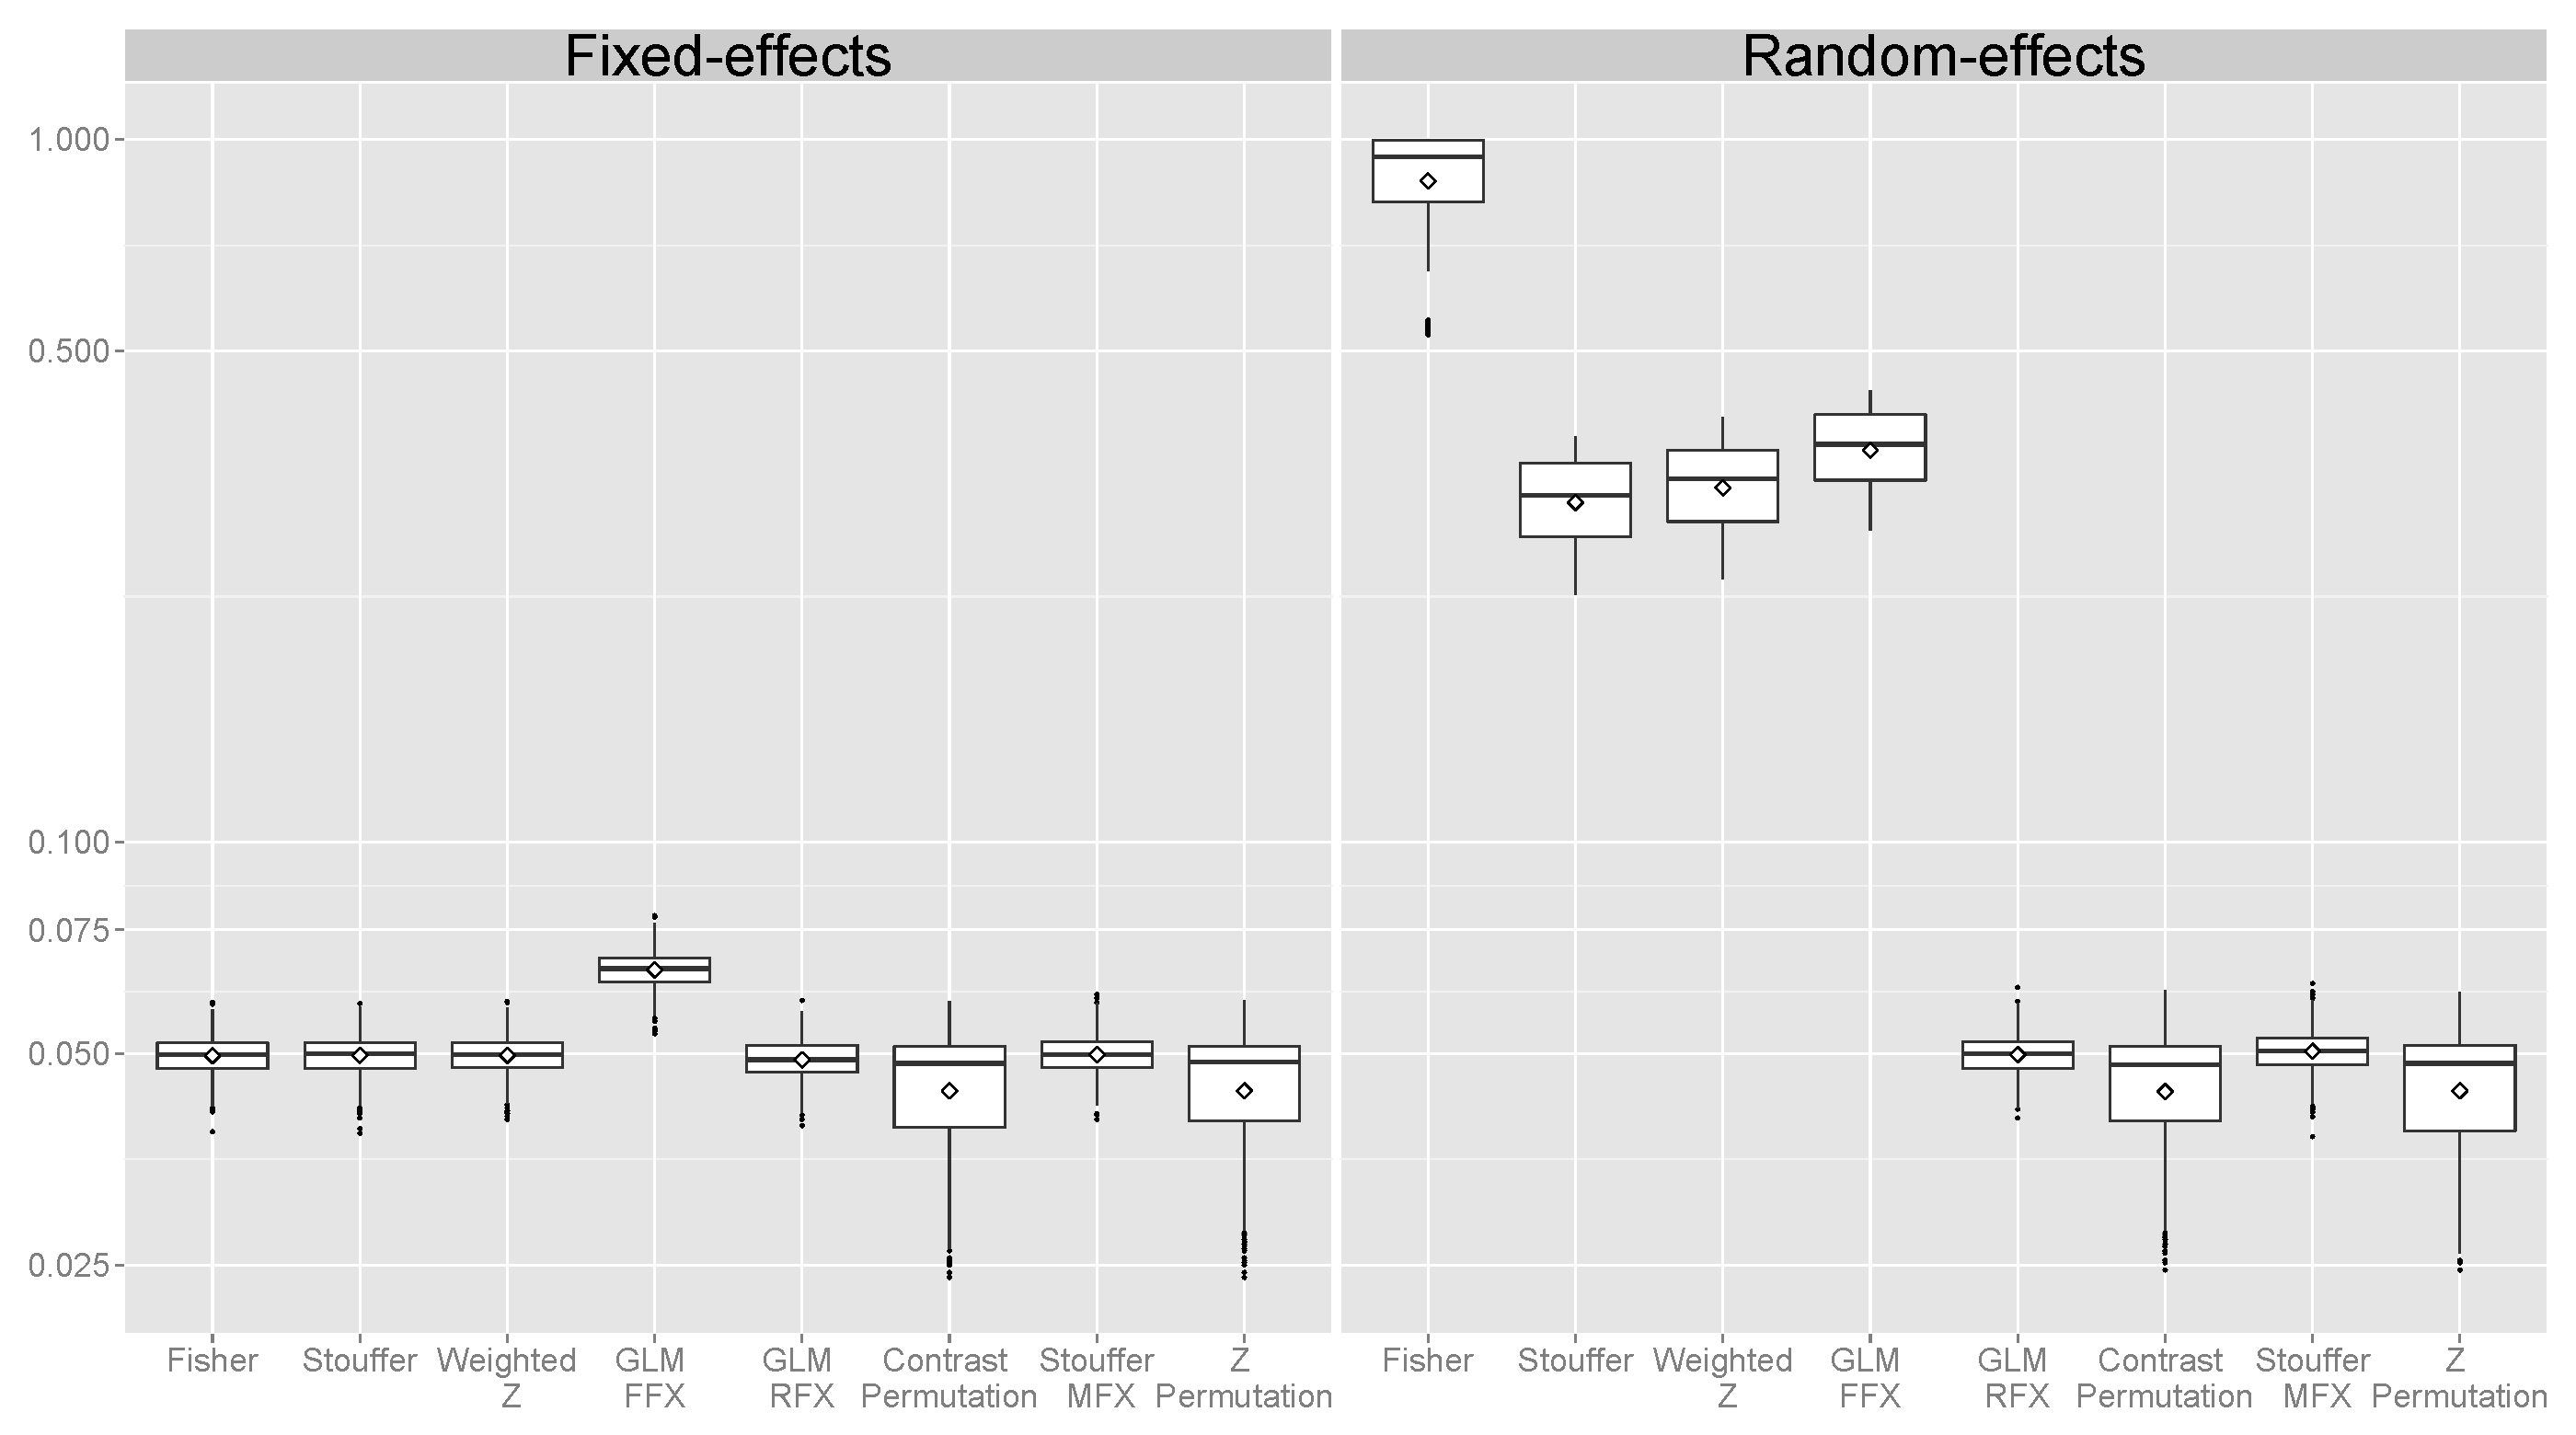
\includegraphics[width=\linewidth]{./Rplot_FPR_all.pdf}
	\caption{False positive rates of the meta-analytic estimators under the null hypothesis for $p<0.05$.}
	\label{fig_fpr_all}
\end{figure}

The impact of the number of studies involved in the meta-analysis and of the size of the within-study variance are investigated in fig.~\ref{fig_fpr_valid}. The permutation estimates appears conservative ($\text{FPR}\simeq 0.03$) when 5 studies are involved. All approaches perform equally as soon as 10 or more studies are included in the meta-analysis. 
\begin{figure}[ht]
	\centering
	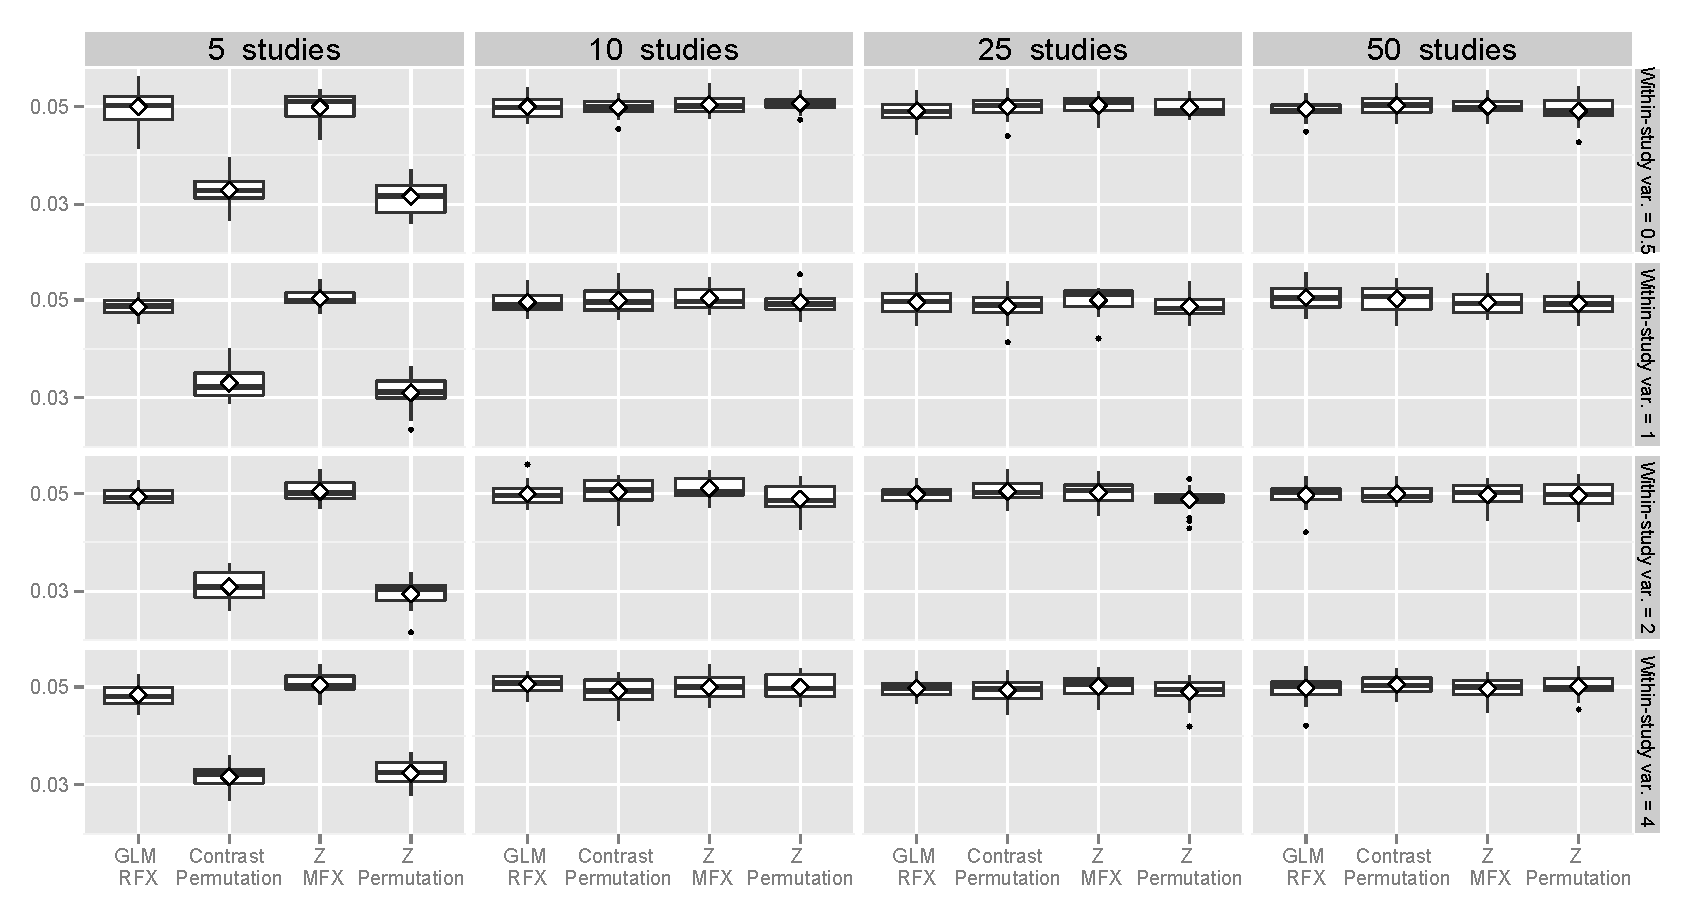
\includegraphics[width=\linewidth]{./Rplot_valids.pdf}
	\caption{False positive rates of the valid random-effects meta-analytic estimators under the null hypothesis for $p<0.05$ as a function of the number of studies and the within-study variance.}
	\label{fig_fpr_valid}
\end{figure}


\subsection{Real data}
Fig. 1 shows the Bland-Altman plots comparing Z-scores from the Stouffer's and weighted-Z methods each compared with the ground truth Z-scores. Overall, both approaches present the same pattern of overestimation of the Z-scores. The weighted-Z approach provides a somewhat more condensed pattern suggesting a closer match to the ground truth.
The dice similarity score for uncorrected p-values of 0.001, 0.01 and 0.05 were 0.84, 0.87 and 0.89 respectively for Stouffer's method and 0.86, 0.88 and 0.90 for the weighted Z-score, showing again slightly better results for the weighted-Z approach. These scores are notably higher (dice similarity scores range from 0 to 1) than the scores obtained with coordinate-based meta-analyses (around 0.5, [5]).
Finally the ROC curves displayed in figure 2 for a ground truth obtained with an FDR corrected threshold p<0.05 demonstrate again a slight advantage of weighted-Z FFX over Stouffer's FFX.

Dice among valids
\begin{enumerate}
\item StouffersMFX: 0.9454
\item PermutZ: 0.9450
\item GLMRFX: 0.8994
\item PermutCon: 0.8991
\end{enumerate}

\begin{enumerate}
\item WeightedZ: 0.9244
\item Stouffers: 0.9184
\item GLMFFX: 0.8972
\item fishers: 0.8382
\end{enumerate}

AUC between 0 and 0.1
among valids
\begin{enumerate}
\item StouffersMFX: 0.8924
\item PermutZ: 0.8919
\item GLMRFX: 0.7809
\item PermutCon: 0.7815
\end{enumerate}

\begin{enumerate}
\item  WeightedZ: 0.8293
\item  Stouffers: 0.8619
\item  fishers: 0.6329
\item  GLMFFX: 0.6111
\end{enumerate}
    

         
       
          
       
    
       

\section{Conclusion}
We have found appreciable differences between the Z-score only approaches as compared to a gold-standard approach. Overall the weighted-Z method provided results that were closer to the ground truth than Stouffer's approach. We hypothesize that Stouffer's methods may be attributing greater weights to less-representative subsets of the data. All three procedures are valid, but the gold-standard should be giving the most faithful representation of the population effect. This advocates over the development of tools supporting the sharing E+SE's.

\section{Acknowledgements}
We gratefully acknowledge the use of this data from the Tracey pain group, FMRIB, Oxford.

%
% ---- Bibliography ----
\bibliographystyle{plain}
\bibliography{miccai2014}

% %
% \begin{thebibliography}{5}
% %
% \bibitem {clar:eke}
% Clarke, F., Ekeland, I.:
% Nonlinear oscillations and
% boundary-value problems for Hamiltonian systems.
% Arch. Rat. Mech. Anal. 78, 315--333 (1982)

% \bibitem {clar:eke:2}
% Clarke, F., Ekeland, I.:
% Solutions p\'{e}riodiques, du
% p\'{e}riode donn\'{e}e, des \'{e}quations hamiltoniennes.
% Note CRAS Paris 287, 1013--1015 (1978)

% \bibitem {mich:tar}
% Michalek, R., Tarantello, G.:
% Subharmonic solutions with prescribed minimal
% period for nonautonomous Hamiltonian systems.
% J. Diff. Eq. 72, 28--55 (1988)

% \bibitem {tar}
% Tarantello, G.:
% Subharmonic solutions for Hamiltonian
% systems via a $\bbbz_{p}$ pseudoindex theory.
% Annali di Matematica Pura (to appear)

% \bibitem {rab}
% Rabinowitz, P.:
% On subharmonic solutions of a Hamiltonian system.
% Comm. Pure Appl. Math. 33, 609--633 (1980)

% \end{thebibliography}


\end{document}
